\chapter{REVISIÓN DE LITERATURA}

\blindmathpaper

\begin{figure}[H] % tiny 
	\centering
	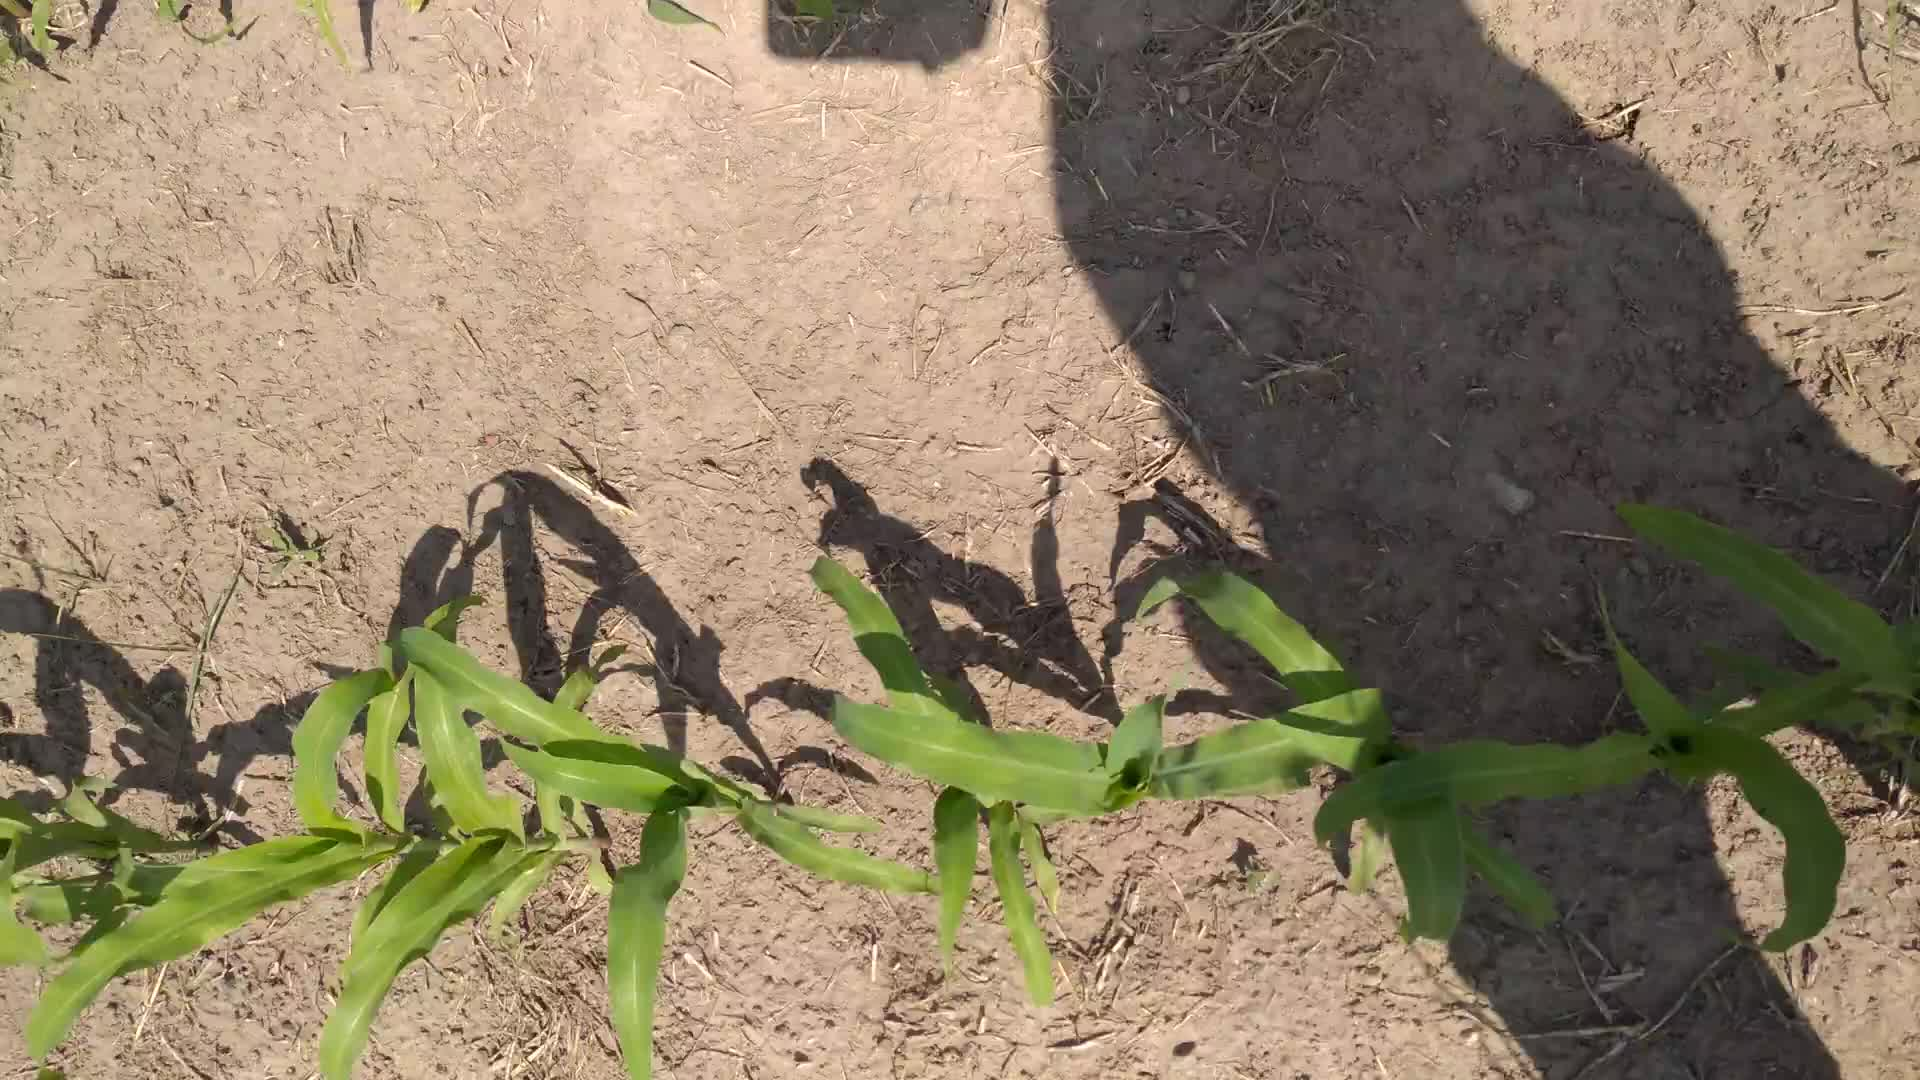
\includegraphics[width=1\textwidth]{Imagenes/0001}
	\caption[Titulo de lista]{Titulo completo}
	\label{fig:yolov4-t}
\end{figure}


\begin{table}[H] % versiones de YOLOv5
	\caption[Versiones de YOLOv5]{Versiones de YOLOv5} \label{tab:Verv5}
	\centering
	\begin{tabular}{lcc}
		\toprule
		\textbf{Versión} & \textbf{Profundidad del modelo} & \textbf{Ancho de capas}\\
		\midrule
		YOLOv5n & 0.33 & 0.25 \\
		YOLOv5s & 0.33 &  0.50 \\
		YOLOv5m & 0.67 & 0.75 \\
		YOLOv5l & 1.00 & 1.00 \\
		YOLOv5x & 1.25 & 1.25 \\
		\bottomrule
	\end{tabular}
\end{table}